

\documentclass[conference]{IEEEtran}
\IEEEoverridecommandlockouts
% The preceding line is only needed to identify funding in the first footnote. If that is unneeded, please comment it out.
\usepackage{cite}
\usepackage{amsmath,amssymb,amsfonts}
\usepackage{algorithmic}
\usepackage{graphicx}
\usepackage{textcomp}
\usepackage{xcolor}
\usepackage{array}
\usepackage{stfloats}
\usepackage{pifont}

\usepackage[noblocks]{authblk}

\usepackage{algorithm}
%\usepackage[ruled,linesnumbered]{algorithm2e} 
%\usepackage{algpseudocode} 
%\usepackage{algorithmicx}    
\renewcommand{\algorithmicrequire}{\textbf{Input:}}  % Use Input in the format of Algorithm
\renewcommand{\algorithmicensure}{\textbf{Output:}} % Use Output in the format of Algorithm 

%缩进提示线





\def\BibTeX{{\rm B\kern-.05em{\sc i\kern-.025em b}\kern-.08em
    T\kern-.1667em\lower.7ex\hbox{E}\kern-.125emX}}

\begin{document}

\title{Hierarchical Time-frequency Synchronization Mechanism for Time Sensitive Networking
%{\footnotesize}
%\thanks{Identify applicable funding agency here. If none, delete this.}
}

\author[ ]{Yunzhu Yu}
\author[*]{Kaijie Wu}
\author[ ]{Qimin Xu}
\author[ ]{Xiang Chen}
\author[ ]{Cailian Chen}
\affil[ ]{Department of Automation, Shanghai Jiao Tong University, Shanghai 200240, P. R. China \authorcr Key Laboratory of System Control and Information Processing, Ministry of Education of China}
\affil[*]{Corresponding Author. Email:Kaijiewu@sjtu.edu.cn}

%\author{\IEEEauthorblockN{1\textsuperscript{st} Yunzhu Yu}
%\IEEEauthorblockA{\textit{dept. name of organization (of Aff.)} \\
%\textit{name of organization (of Aff.)}\\
%Shanghai, China \\
%YuYunzhu@sjtu.edu.cn}
%\and
%\IEEEauthorblockN{2\textsuperscript{nd} Kaijie Wu}
%\IEEEauthorblockA{\textit{dept. name of organization (of Aff.)} \\
%\textit{name of organization (of Aff.)}\\
%Shanghai, China \\
%email address or ORCID}
%\and
%\IEEEauthorblockN{3\textsuperscript{rd} Given Name Surname}
%\IEEEauthorblockA{\textit{dept. name of organization (of Aff.)} \\
%\textit{name of organization (of Aff.)}\\
%City, Country \\
%email address or ORCID}
%}

\maketitle

\begin{abstract}
Modern Industrial Internet-of-Things (IIoT) requires reliable interaction and integration of data in the network. Thus, time sensitive networking (TSN) is a promising technology due to deterministic latency guarantee mechanisms for data transmission. However, the multiple mechanisms are based on the networkwide precise time synchronization. In this paper, to achieve precise and reliable clock synchronization of TSN, we propose a hierarchical timing-frequency synchronization mechanism. Specifically, the network is divided into two layers according to the network clock synchronization function. The top layer adopts tree-based synchronization to provide a global clock and an interface with external standard clock synchronization, and the underlying one adopts a distributed synchronization protocol to improve the reliability, which obtains the reference clock by multiple nodes to avoid the single point of failure. To improve synchronization efficiency, a time-frequency fusion synchronization mechanism is proposed, which comprehensively considers the synchronization time slot difference and the time-frequency coupling relationship to improve the synchronization speed under the same synchronization period. Simulation results show that the proposed synchronization mechanism has higher synchronization efficiency than the traditional methods, and improves the clock synchronization speed and accuracy significantly.
\end{abstract}

\begin{IEEEkeywords}
Clock synchronization, Time sensitive networking, Precision time protocol (PTP), AS6802
\end{IEEEkeywords}

\section{Introduction}
With the introduction of Industry 4.0, smart factories have become a new stage of modern factory informatization development \cite{ref15}. Smart factories realize the cluster interaction of different types of industrial data through the Industrial Internet-of-Things (IIoT) and promote the intelligent and networked transformation and upgrading of manufacturing through data fusion \cite{ref18}. The precise interaction and fusion of data need to ensure that data is transmitted within a specific limited time. It requires the network to be deterministic and real-time, which are also the most important characteristics of industrial networks \cite{ref19}. Although there are currently deterministic Ethernet protocols, such as Profinet \cite{ref29}, EtherCAT \cite{ref30}, Ethernet Powerlink \cite{ref32}, etc., they cannot achieve deterministic transmission under mixed data streams. So the IIoT based on these protocols cannot guarantee the accuracy and reliability of the data. To improve the real-time performance and reliability of Ethernet with mixed data, the IEEE 802.1 task group began the research on Time Sensitive Networking (TSN) \cite{ref21}.

TSN is considered as a universal communication tool under Industry 4.0 \cite{ref23}, extending the traditional Ethernet data link layer standard to ensure that data transmission has limited ultra-low latency and low jitter \cite{ref22}. Clock synchronization provides a general and accurate time for all TSN devices, which is the basis of TSN. Without precise clock synchronization, TSN is not able to control the gate switch in the Gate Control Lists (GCL) at an accurate time during the flow schedule, affecting the deterministic delay of TSN. Therefore, TSN puts forward significant requirements for clock synchronization accuracy and reliability between devices.

Aiming at the problem of clock synchronization, effective methods have been proposed in previous studies. In terms of synchronization structure, the current mainstream methods mainly include tree-based synchronization and distributed synchronization \cite{ref24}. 

The tree-based protocol needs to establish a hierarchical structure in the network, which includes a master node and other slave nodes. Typical representatives are the network time protocol (NTP) \cite{ref25}, the precise time protocol (PTP) \cite{ref2} and IEEE 802.1AS generalized precision time protocol (gPTP) \cite{ref28}. NTP implements Internet synchronization at the application layer, with low synchronization accuracy due to errors generated by the network protocol stack. PTP obtains time stamps at the location between the physical layer and the MAC layer, which improves synchronization accuracy. gPTP is developed based on PTP, which uses a two-step delay measurement. Although tree-based synchronization is simple to implement, errors will occur in each level of synchronization. As the network scale increases, errors will continue to accumulate, which seriously affects the synchronization performance.

Distributed synchronization is different from tree-based synchronization. The clock reference is not provided by a master node but determined by multiple nodes in the network. AS6802 \cite{ref3} is a typical distributed synchronization protocol, which is mainly applied to aviation networks. Due to the distributed structure, the network avoids the hierarchical structure and reduces the cumulative errors \cite{ref24}. Since the reference clock is not entirely dependent on one node, the reliability of synchronization is significantly improved compared to tree-based. However, due to the lack of nodes synchronized with the external clock, synchronization can only be performed within the network, and local clock synchronization causes the internal clock to shift overall and cannot synchronize with Coordinated Universal Time (UTC).

%In master-slave synchronization, a global master clock is selected as the Grandmaster (GM) in the network, and then the GM is synchronized with the clock of the next level. The next level of clock must adjust its local clock to synchronize with the GM. The next clock is then used as the master clock for the clock lower than it to perform master-slave synchronization. This synchronization method is a typical serial synchronization. Typical representatives are the network time protocol (NTP) \cite{ref4} in traditional Ethernet and the precise time protocol (PTP) \cite{ref5} in industrial control. Although the master-slave synchronization is simple to implement, errors will occur in each level of master-slave synchronization. As the network scale increases, this error will continue to accumulate, which seriously affects the synchronization performance. Although PTP proposes the concept of a transparent clock to reduce this cumulative error, PTP depends on the support of special hardware to ensure its own synchronization accuracy, which limits its application. At the same time, because the master-slave synchronization relies heavily on the clock accuracy of the master clock, even if a new GM fails, the reliability of the synchronization will be reduced and the synchronization time will be increased.

%However, distributed synchronization effectively solves the problem of error accumulation. Unlike master-slave synchronization, it does not have a master clock concept. Instead, multiple devices in the network are selected and the average value of a clock is obtained by calculating the clocks of these devices as the clock reference for the whole network. AS6802 is a typical distributed synchronization method, which is mainly suitable for aviation networks. Because of the distributed structure, there is no cumulative error, and because not entirely rely on a device to obtain the clock benchmark, also greatly improve the reliability of synchronization. However, due to the lack of equipment to synchronize with the external clock, the synchronization with UTC can not be realized, only the synchronization within the network.

The above synchronization protocols are essentially time synchronization. Besides time synchronization, clock synchronization also includes frequency synchronization \cite {ref4}. In practical applications, the clock frequency is time-varying due to the effects of temperature \cite{ref4}, aging \cite{ref27}, etc., resulting in continuous errors in the clock after the long-term operation, so the frequency offset cannot be ignored for high precise \cite{ref26}. Therefore, frequency synchronization is required to improve the accuracy of clock synchronization, especially in a harsh industrial environment.

Some existing works have investigated the synchronization of frequency offset. For example, for multi-hop wireless sensor networks, Wang et al. \cite{ref9} studied a time synchronization scheme and a corresponding clock frequency estimation method, assuming that the noise is a Gaussian model. Fan et al. \cite{ref10} realized simultaneous synchronization of time and frequency by using a parametric differential clock synchronization algorithm. Zhang et al. \cite{ref11} proposed a new clock synchronization scheme based on maximum consistency for wireless sensor networks. However, the above methods are complicated and require frequent timing information exchange between nodes, resulting in longer calculation time and ultimately affecting the low-latency characteristics of TSN. Hence, the study of frequency synchronization without increasing the computational complexity is an important research topic.

%In order to eliminate clock synchronization errors caused by clock frequency drift, Moon et al. \cite{ref9} proposed a method to calculate the clock frequency ratio of the transmitting and receiving ends. By measuring the time difference between the transmitting and receiving ends of the probe packet in a large amount, the conditional extreme value theory was used to analyze the measurement data and the clock frequency difference of the clocks at both ends was estimated by directly measuring the delay slope. Many subsequent studies were completed on the basis of Moon. For multi-hop wireless sensor networks, Wang et al. \cite{ref22} Studied a time synchronization scheme with instant clock adjustment and a corresponding clock frequency estimation method assuming that the noise is a Gaussian model. Fan et al. \cite{ref10} established a logical clock model for parallel distributed systems, and realized synchronous synchronization of time and frequency by using parametric differential clock synchronization algorithm. Wang et al. \cite{ref12} proposed a time-frequency synchronization algorithm similar to maximum likelihood estimation for semi-phase multi-entry and multi-exit systems, and used grid search to jointly estimate the starting time and frequency deviation. Zhang et al. \cite{ref14} proposed a new clock synchronization scheme based on maximum consistency for wireless sensor networks considering bounded noise at the same time. 

%However, TSN has to deal with a larger and more complex network, which requires synchronization to have both high accuracy and high reliability in the face of complex network environments. Most of the above-mentioned time-frequency synchronization methods are based on master-slave synchronization, which has relatively low reliability and is not suitable for complex networks. This requires us to design a synchronization mechanism that can achieve time-frequency synchronization to ensure synchronization accuracy and improve reliability.

%Motivated by these, the main work of this paper is to propose a double-layer clock synchronization mechanism for TSN. The network is divided into two layers based on existing synchronization protocols. The top network uses tree-based synchronization to provide a global clock and external interface to the network. The underlying network uses a distributed structure and relies on multiple nodes to provide reference clocks to improve network reliability. The two layers of the network use the Synchronization Master (SM) as the interface for information exchange and synchronizes time and frequency simultaneously. Synchronization information is transmitted between the two layers of the network at different times, which can reduce the pressure of calculation and control. The proposed synchronization mechanism can be implemented on the existing protocols. Finally, based on the OMNET++ simulation, a TSN network transmission system was constructed, and the performance of clock synchronization accuracy was verified. The contributions of this paper are threefold:

Motivated by these, the main work of this paper is to propose a hierarchical time-frequency synchronization mechanism for TSN. The main contributions of this work are as follows.

\begin{itemize}
	
	\item A hierarchical synchronization mechanism was established to improve synchronization reliability, in which the reference clock is calculated in a distributed multi-node collaborative decision mode to avoid the single point failure of the reference clock.
	\item To improve synchronization efficiency, a time-frequency fusion synchronization mechanism is proposed. Considering the synchronization time slot difference and the time-frequency coupling relationship, the offset of time and frequency are cooperatively regulated to improve the synchronization speed under the same synchronization period.
	
\end{itemize}
 
The main structure of this work is as follows. The second part is the clock model. The third part introduces the hierarchical synchronization mechanism proposed in this paper. The fourth part validates the effectiveness of the proposed mechanism through experiments. The fifth part is the conclusions. 

\section{Clock Model}

The clock of network equipment is usually driven by a quartz crystal oscillator. The oscillator drives a counter which is filled with a constant value beforehand. When the oscillator sends a pulse, the counter is decremented by one until it reaches zero, and the clock is driven to generate a tick. The constant value is refilled into the counter and reloaded after that, repeating the above operation process \cite{ref12}.

We assume the time of the reference clock is $C(t)=t$, where $t$ is the reference time with a frequency of $1$. After a synchronization period $t_0$, a typical quartz-stabilized oscillator clock model of node $i$ is,

\begin{equation}
C_i(t_0) = \Delta_i  + \int_0^{t_0} {f_i(t)dt}, \label {eq1}
\end{equation}

\noindent where $C_i(t_0)$ and $f_i(t)$ is the clock time and real clock frequency of node $i$, respectively. $\Delta_i$ represents the initial clock offset between node $i$ and the reference clock.

In practical applications, $f_i(t)$ is not a fixed value, and it will be affected by many factors, including initial errors and random errors caused by temperature and oscillator aging, etc. \cite{ref4, ref27}. So we can get the expression of the clock frequency of node $i$, %The internal factors from the equipment include the initial error between the quartz crystal oscillator during the manufacturing process and the nominal frequency at the factory, and the aging error caused by the aging of the oscillator \cite{ref23}. External natural environmental errors include temperature and pressure, humidity, and vibration. But errors caused by pressure, humidity and vibration can be eliminated by the package of the oscillator \cite{ref3}. Therefore, the external factor that has the greatest effect on the frequency of the oscillator is temperature. So we can get the expression of the clock frequency of node $i$,

%\begin{equation}
%f_i(t) = F_i + \delta_i  + \omega_i(t) + \phi_i(T) \label {eq2}
%\end{equation} 

%Where $F_i$ is the nominal frequency. $\delta_i$ is the initial errors after delivery due to manufacturing process errors, etc. of the oscillator. $\omega_i(t)$ and $\phi_i(T)$ are frequency error functions due to aging of the oscillator and temperature changes in the natural environment. For simplicity, we can consider the error caused by temperature as a random variable. As the oscillator runs longer, the random variable follows a normal distribution with a mean value of $0$ and a variance of $\sigma^2$. The error due to the aging of the oscillator is very small and ignored in the analysis of this article. As for initial random errors, we assume that the maximum value is $\rho$, that is, $- \rho \le \delta_i \le + \rho$. Then,

\begin{equation}
f_i(t)=F_i+\delta_i+\phi_i, \label {eq2}
\end{equation}

\noindent where $F_i$ is the nominal frequency. $\delta_i$ is the initial errors after delivery due to manufacturing process errors, etc. of the oscillator. We assume that the maximum value is $\rho$, that is, $- \rho \le \delta_i \le + \rho$. $\phi_i \sim \mathcal N(0,\sigma^2)$.

%Under the existing PTP protocol, the frequency variation in the model is mainly ignored, and only the estimated value of the time offset is calculated. Under the AS6802 protocol, the frequency is also ignored, and only the time average of multiple nodes is calculated. These cause the calculated time offset or time average to be different from the current offset after synchronization for a period of time, leading to a decrease in synchronization accuracy. So we consider simultaneously performing frequency and time synchronization during the synchronization process. Although there is an error in the initial time synchronization, the nodes in the network can quickly reach the synchronized state. Frequency synchronization takes a little time, but after several frequency synchronizations between nodes, the error will be significantly reduced when time synchronization is performed.

\section{Proposed Hierarchical Timing-frequency Synchronization Mechanism}
%In this section, we propose a double-layer timing-frequency synchronization mechanism. Next, we will introduce our synchronization mechanism. 

\begin{figure}[htbp]
	\centerline{\includegraphics[scale=0.45]{fig1.eps}}
	\caption{Network hierarchy structure.}
	\label{fig1}
\end{figure}

We divide the nodes in the network into the following categories: Grand Master (GM), Frequency Master (FM), Synchronization Master (SM), Compression Master (CM), and Synchronization Client (SC). The network is divided into two layers according to the network clock synchronization function. In terms of synchronous structure, the top network and underlying network adopt tree-based and distributed architectures, respectively. The hierarchical network structure is shown in Fig. 1. The two layers of the network use the SM and FM as the interface for information exchange, and time-frequency synchronize. We define a time synchronization period $P_t$ as a period for performing a time offset correction and a frequency synchronization period $P_f$ as a period for performing a frequency offset correction. A frequency synchronization period consists of multiple time synchronization periods.

%\renewcommand\arraystretch{1.5}

%The cluster period mentioned below is defined as the traffic that requires the highest transmission delay of each pair in the network, that is, the least common multiple of the time-critical flow scheduling period, such as the time-triggered flow of TTE networks and TSN networks. The integration period mentioned below is a clock synchronization period. The relationship between the cluster period and integration period is: $Integration \  period = \frac {Cluster \  period} {N}$, $N$ can be any positive integer.

%At the beginning of each time synchronization period, all devices except the GM send the local clock information of each device to the GM. GM defines the device with the most stable clock frequency as Frequency Master (FM). 

%After that, GM will cluster the devices in the network according to the principle of close clocks. If a device has the most devices in the cluster, the device is an Synchronization Master (SM). Then set several Compression Master (CM) at the same time, guarantee the SM to CM minimum hop count, the rest of the equipment is Synchronization Client (SC).

\subsection{Top Network Synchronization Mechanism Design}\label{AA} 

%\paragraph{Master-Slave Time Synchronization}
The top network refers to PTP and uses the tree-based synchronization mechanism. The specific process is as follows.

\begin{figure}[htbp]
	\centerline{\includegraphics[scale=0.5]{fig2.eps}}
	\caption{Top network time synchronization process, $D_{ms}$ and $D_{sm}$ are represent downstream delay and upstream delay, respectively.}
	\label{fig2}
\end{figure}

We assume that the master and slave nodes have the same frequency and are fixed, then,

%\begin{equation}
%T_s = T_m + \Delta, \label {eq3}
%\end{equation}

%\noindent Where $ \Delta $ is the clock offset. The actual values (that is, the time relative to the master clock) of the uplink delay (the transmission delay from the slave to the master) and the downlink delay (the transmission delay from the master to the slave) are,

%\begin{equation}
%\left\{ {\begin{array}{*{20}{c}}
	%{{D_{ms}} = T_s^1 - T_m^1 - \Delta }\\
	%{{D_{sm}} = T_m^2 - T_s^2 + \Delta }
	%\end{array}} \right.
%\label {eq4}
%\end{equation}

%Assuming that the uplink delay and downlink delay are fixed and constant, calculate the one-way delay $D_w$ and clock offset $\Delta$:

%\begin{equation}
%{D_w} = \frac{{{D_{ms}} + {D_{sm}}}}{2} = \frac{{({T_s^1} - {T_m^1}) + ({T_m^2} - {T_s^2})}}{2} \label{eq5}
%\end{equation}

\begin{equation}
\Delta  = \frac{{(T_s^1 - T_m^1) - (T_m^2 - T_s^2)}}{2}, \label{eq3}
\end{equation}

\noindent where $ \Delta $ is the clock offset.

In this way, the time offset between the master and slave nodes is calculated. In our top network, we set GM as the master node and SM as the slave node. At the same time, we take into account the frequency variation between nodes and adopt frequency synchronization to correct the frequency offset. We use the method shown in Fig. 3 to synchronize the frequency.

%\paragraph{Master-Slave Frequency Synchronization}
%FM and GM adopt master-slave frequency synchronization while SM and GM perform master-slave time synchronization. GM sends data to FM while sending the information to SM, and FM records the transmission delay from GM. As shown in the Figure 5, we analyze the principle of master-slave frequency synchronization.

\begin{figure}[htbp]
	\centerline{\includegraphics[scale=0.5]{fig3.eps}}
	\caption{Top network frequency synchronization process, $D_i$ is the actual one-way delay (master to slave) of the detection packet and $d_i$ is the measured one-way delay of the detection packet.}
	\label{fig3}
\end{figure}

The sending time of the probe packet $i$ at the master is $T_m^i$, and at the same time, the time of the slave is $T_s^i$; The time when the probe arrives at the slave is $T_s^{i'}$, and at the same time, the time of the master is $T_m^{i'}$.

Assume that the clock offset of the master and the slave at the beginning of the measurement is $\Delta_0$, and $\Delta_0 = T_s^1 - T_m^1$. Assume that the clock frequency of the master is $f_m$, and the clock frequency of the slave is $f_s$. The ratio of the master clock to the slave clock is $\alpha$. Then,

%\begin{equation}
%T_s^1 = T_m^1 + \Delta_0 \label {eq7}
%\end{equation}

%\begin{equation}
%T_s^i - T_s^1 = \frac{{{f_m}}}{{{f_s}}}(T_m^i - T_m^1) = \alpha (T_m^i - T_m^1) \label {eq8}
%\end{equation}

\begin{equation}
\alpha = \frac{{{f_m}}}{{{f_s}}} = \frac{F_m+\delta_m+\phi_m}{F_s+\delta_s+\phi_s}. \label {eq4}
\end{equation}

%In section II, we analyzed the model of the clock frequency. We can have,

%\begin{equation}
%\alpha = \frac{F_m+\delta_m+\phi_m}{F_s+\delta_s+\phi_s} \label {eq9}
%\end{equation}

The measured one-way delay $d_i$ is,

\begin{equation}
\begin{aligned}
d_i &= T_s^{i'} - T_m^i = T_s^i + \alpha {D_i} - T_m^i\\
 	&= T_s^1 + \alpha (T_m^i - T_m^1) + \alpha {D_i} - T_m^i + (T_m^1 - T_m^1)\\
 	&= (\alpha  - 1)(T_m^i - T_m^1) + \Delta_0  + \alpha {D_i} 
\end{aligned},
\label{eq5}
\end{equation}

%\begin{equation}
%\begin{aligned}
%d_i &= T_s^{i'} - T_m^i = T_s^i + \alpha {D_i} - T_m^i\\
	%&= (\alpha  - 1)(T_m^i - T_m^1) + \Delta_0  + \alpha {D_i} 
%\end{aligned},
%\label{eq10}
%\end{equation}

\noindent where $D_i=T_m^{i'}-T_m^i$. Because the clock frequency offset is generally not greater than $10^{-4}$, and the one-way delay is usually in the millisecond range, $d_i$ can be simplified as,

\begin{equation}
d_i = (\alpha - 1)(T_m^i - T_m^1) + \Delta_0 + D_i. \label {eq6}
\end{equation}

When the network structure does not change, it can be considered that the value of $D_i$ is stable. At this time, it can be regarded as that the changing trend of $d_i$ is determined by $\alpha$, that is, the clock frequency offset can be calculated by measuring the delay and used to compensate.

In practical applications, we use GM as the master node and FM as the slave node. When GM sends data to SM, GM starts to synchronize the data to FM at a fixed time interval. The frequency offset is calculated according to formula (6), where $\Delta_0$ can be approximately the time offset calculated by the first time synchronization period.

%Considering that the clock frequency difference will change over time, we can use parameter identification to calculate the current clock frequency difference online in real time. The calculation of the changed clock frequency difference has nothing to do with the data before the change. The slope of the data is gradually changing. The recursive least squares of fuzzy or piecewise forgetting factors reduces the association with old data.

\subsection{Underlying Network Synchronization Mechanism Design}\label{BB}

%\paragraph{Distributed Time Synchronization}
After completing the clock synchronization with GM, SM enters the distributed time synchronization stage, generates frames that contain their clock information, and sends them to CM. This process refers to the AS6802 protocol.

After receiving the data sent by SM, CM obtains several permanence points through the permanence operation. During this stage, the required permanence point is obtained after collection. The permanence point is obtained by,

\begin{equation}
p{p_i} = d_{max} + r{p_i} - d_i, \label {eq7}
\end{equation}

\noindent where $pp_i$ corresponds to the $i$-th collected permanence point. $d_{max}$ is the maximum transmission delay in the network which can be defined in advance or measured experimentally. $r{p_i}$ is the time point when CM received the data, and $d_i$ represents the data transmission delay in the link.

Then we can have ${{p_i} = p{p_i} - p{p_1}}$, where $p_i$ corresponds to the time difference between the $i$-th collected permanence point and the first permanence point. The following formula is taken to calculate the compression correction value $corr$:

%\begin{equation}
%\left\{ {\begin{array}{*{20}{l}}
	%{k = 1,corr = {p_1}}\\
	%{k = 2,corr = \frac{{{p_1} + {p_2}}}{2}}\\
	%{k = 3,corr = {p_2}}\\
	%{k = 4,corr = \frac{{{p_2} + {p_3}}}{2}}\\
	%{k = 5,corr = \frac{{{p_2} + {p_4}}}{2}}\\
	%{k > 5,corr = \frac{{{p_f} + {p_{k - f}}}}{2}}
	%\end{array}} \right.,
%\label {eq8}
%\end{equation}

\begin{equation}
\left\{ {\begin{array}{*{20}{l}}
{0 < k \le 5,corr = \frac{{{p_f} + {p_{k - f + 1}}}}{2}}\\
%{k = 3,corr = {p_2}}\\
%{k = 4,corr = \frac{{{p_2} + {p_3}}}{2}}\\
%{k = 5,corr = \frac{{{p_2} + {p_4}}}{2}}\\
{k > 5,corr = \frac{{{p_f} + {p_{k - f}}}}{2}}
\end{array}} \right.,
\label {eq13}
\end{equation}

\noindent where $k$ corresponds to the number of collected permanence points; $f$ is the maximum number of SMs allowed to error in the network. If $0<k\le2$, $f=1$, and if $2<k\le5$, $f=2$.

After calculating the $corr$ based on the received frames, CM generates a new frame and send it to GM, SM, FM, and SC. They adjust the local clock after receiving the frame sent by CM. This process completes the time synchronization of a time synchronization period.

We also use FM as the starting node and use synchronous Ethernet technology to transform some nodes of the underlying network and add clock phase-locked loop modules (PLL). In this way, FM injects the clock synchronized with GM into its physical layer and sends it to other nodes through the network. The other nodes act as relay nodes and continue to send clocks to other nodes. All nodes can restore the clock frequency based on the received data. This process completes the frequency synchronization of a frequency synchronization period. The specific synchronization process of the underlying network is shown in Fig. 4.

\begin{figure}[h]
	\centerline{\includegraphics[scale=0.6]{fig4.eps}}
	\caption{Underlying network clock synchronization process.}
	\label{fig4}
\end{figure}

%\paragraph{Distributed Frequency Synchronization}
%FM process the data transmission delay measurement value sent by GM within a cluster period to process the clock frequency offset. Then FM adjust its local clock frequency. The subsequent frequency values are sent to SM, CM, and SC. They adjusts their local clock frequency according to the received frequency adjustment information.

%We assume that the clock of each device is maintained by a phase lock. Once the frequency of FM remains the same after synchronizing with GM, the frequency can be sent to all devices through synchronous Ethernet technology \cite{ref26}. The phaser adjusts its own clock frequency and keeps it. The specific process is shown in Figure 7.

%\begin{figure}[htbp]
	%\centerline{\includegraphics[scale=0.45]{fig5.eps}}
	%\caption{Distributed frequency synchronization process.}
	%\label{fig5}
%\end{figure}

\subsection{Hierarchical Network Connection Mechanism Design}\label{CC}
The top and underlying network use SM and FM as interfaces. SM and FM are responsible for time and frequency synchronization, respectively. At the end of each $P_f$, GM needs to send its local clock information to CM, which is compared with the underlying network clock reference calculated by the CM. If CM does not receive data from GM or the time offset between them is bigger than a preset threshold $\zeta$, GM is considered to be in an abnormal state.

If GM is in the abnormal state, SM directly adopts distributed synchronization, and FM uses its frequency as the reference for frequency synchronization. Otherwise, SM continues to perform tree-based time synchronization with GM, and FM also adjusts the local frequency according to the frequency of GM. The processing of SM, CM, and FM can be summarized as the following three algorithms.


\begin{algorithm}[ht]  
	\caption{SM clock synchronization process in a $P_f$ period}  
	\begin{algorithmic}[1]
		\REQUIRE Time stamp sent by GM, $T_m^1$ and $T_m^2$; Local time stamp of SM, $T_s^1$ and $T_s^2$; Time correction value sent by CM, $corr$; Frequency sent by FM, $f_{FM}$; GM status $GS$;
		\ENSURE Local time information of SM, $T_{SM}'$;
		\WHILE {$time \in P_f$}
			\WHILE {$time = nP_t, n=1,2\ldots $}
				\IF {$GS$ = normal}
					\STATE GM exchanges information with SM, and SM gets $T_s^1$ and $T_s^2$;
					\IF {receives $T_m^1$ and $T_m^2$}  
						\STATE SM adjusts local time with $\Delta = [(T_s^1 - T_m^1) - (T_m^2 - T_s^2)]/2$;
					\ENDIF
				\ENDIF
				\STATE SM sends $T_{SM}'$ to CM;
				\IF {receives $corr$}
					\STATE SM adjusts local time;
				\ENDIF
				\IF {$time+P_t>P_f$ \textbf{and} receives $f_{FM}$}
					\STATE SM adjusts local frequency;
				\ENDIF
			\ENDWHILE
		\ENDWHILE
		%\RETURN $T_{SM}'$.
	\end{algorithmic}
\end{algorithm}


\begin{algorithm}[ht]  
	\caption{CM clock synchronization process in a $P_f$ period}  
	\begin{algorithmic}[1]
		\REQUIRE Time information sent by GM, $T_{GM}$; Time information sent by SM, $T_{SM}'$; Local time information of CM $T_{CM}$; Frequency sent by FM, $f_{FM}$; Preset threshold, $\zeta$;
		\ENSURE Time correction value $corr$; GM status, $GS$;
		\WHILE {$time \in P_f$}
			\WHILE {receives $T_{SM}'$}
				\STATE CM calculates $corr$ and adjusts local time;  
				\STATE CM sends $corr$ to FM, SM and SC;
				\IF {$time+P_t>P_f$}
					\IF {receives $f_{FM}$}
						\STATE CM adjusts local frequency;
					\ENDIF
					\STATE $GS = abnormal$;
					\IF {receives $T_{GM}$ \textbf{and} $\left| T_{GM} - T_{CM}\right|  \le \zeta$}
						\STATE $GS = normal$;
					\ENDIF
				\ENDIF
			\ENDWHILE
		\ENDWHILE
		%\RETURN $corr$, $GS$.
	\end{algorithmic}
\end{algorithm}


\begin{algorithm}[ht]  
	\caption{FM clock synchronization process in a $P_f$ period}  
	\begin{algorithmic}[1]
		\REQUIRE Time information sent by GM, $T_{GM}'$; Time correction value sent by CM, $corr$; GM status, $GS$;
		\ENSURE Local frequency information of FM, $f_{FM}$;
		\WHILE {$time \in P_f$}
		\REPEAT
		\IF {$GS$ = normal}
		\IF {receives $T_{GM}'$}
		\STATE FM calculates frequency offset and adjusts local frequency;
		\ENDIF
		\IF {receives $corr$}
		\STATE FM adjusts local time;
		\ENDIF
		\ENDIF
		\UNTIL {$time+P_t>P_f$}
		\STATE FM generates $f_{FM}$ and injects it into the network;
		\ENDWHILE
		%\RETURN $f_{FM}$.
	\end{algorithmic}
\end{algorithm}

%The synchronization mechanism proposed in this paper combines tree-based and distributed synchronization. GM mainly provides an interface for the network to communicate with the external standard clock and synchronizes with SM. The underlying network clock reference is essentially a fault-tolerant mean provided by multiple SMs. Since all SMs are synchronized with GM, the clock reference of the underlying network is the same as GM and the calculation of the underlying network can eliminate the random errors caused during synchronization. Because the effect of the frequency offset is also taken into account during synchronization, the synchronization error will be smaller.

%Once GM fails, the underlying network clock reference calculated by CM will be far away from the GM clock. Then the GM clock will be discarded, and the clock reference will directly adopt the clock value calculated by CM. Since SM has been synchronized with GM, the underlying clock reference and the actual clock of GM will not deviate significantly. So that even if a failure occurs, the reliability of the synchronization system can still be guaranteed.

\section{Performance Evaluation}

In this section, we investigate the effectiveness of our proposed hierarchical clock synchronization mechanism. A network structure was built in OMNET++ to verify the performance, as shown in Fig. 5. We first remodeled the clock in OMNET++ according to the mathematical model of the clock (1) and (2) established in section II. The frequency of GM is set to $1$MHz. Set the parameters of all other nodes to $\Delta_0=20$ppm, $F_i=1$MHz, $\delta=20$ppm, and $\phi_i \sim \mathcal N(0,{0.1}^2)$. We choose the SC node as the comparison node and set the bandwidth of all links to $100$M. The propagation delay of all links is set to $25$ns. Then the proposed mechanism is compared with the gPTP in terms of synchronization accuracy and speed.

\begin{figure}[h]
	\centerline{\includegraphics[scale=0.8]{fig5.PNG}}
	\caption{Network structure in OMNET++.}
	\label{fig5}
\end{figure}

\subsection{Synchronization Accuracy}
Fig. 6 shows the tendency of the synchronization errors over time when using the synchronization mechanism we proposed and gPTP with $P_t=2$s. From Fig. 6, one can see that the synchronization errors of gPTP produce large fluctuations due to the influence of frequency offset, and errors of our proposed mechanism change steadily. Under our proposed mechanism, the errors are lower than those under gPTP. The results imply the effectiveness of our mechanism. The frequency offset can cause cumulative time errors, resulting in poor performance. Our proposed mechanism synchronizes the frequency and eliminates errors caused by frequency offset.

\begin{figure}[htbp]
	\centerline{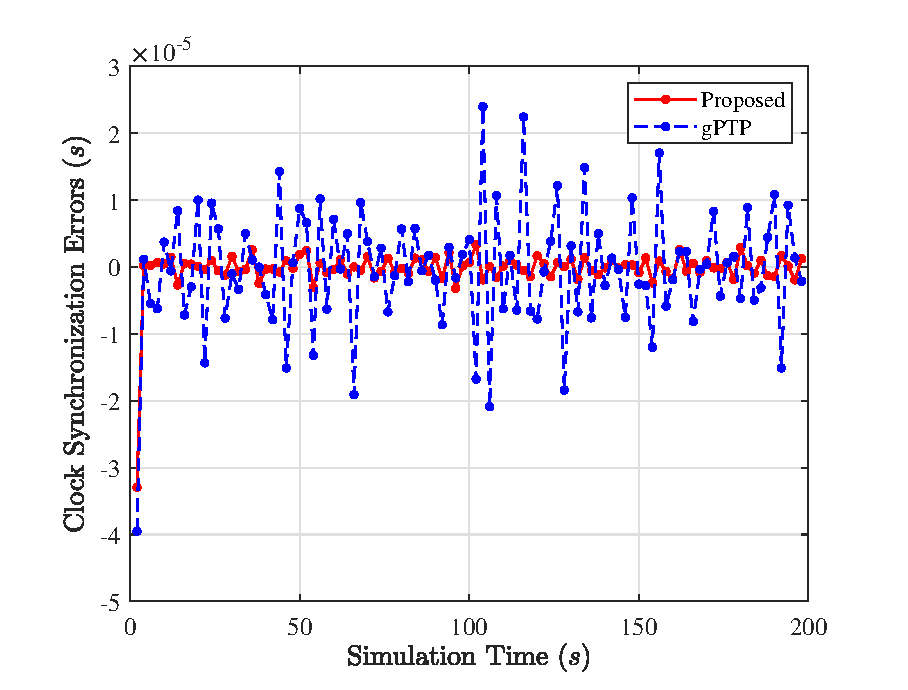
\includegraphics[scale=0.6]{fig6.eps}}
	\caption{Synchronization process comparison of two methods when $P_t=2$s.}
	\label{fig6}
\end{figure}

Fig. 7 shows the synchronization errors that our proposed mechanism and gPTP can achieve with different $ P_t $. The box plot in the figure is the synchronization errors obtained with the increase of simulation time in each period. The line in the figure and the small graph are the medians of the synchronization errors obtained with different $ P_t $. We can see that with the same $P_t$, the errors of the proposed mechanism is smaller than that of gPTP, which means our proposed mechanism can maintain high synchronization accuracy. As the $P_t$ decreases, this difference also decreases. This is because as $ P_t $ decreases, the errors caused by the frequency offset gradually decrease, and the gPTP errors also become smaller. Furthermore, from the box plot in the figure, we can see that the errors of the proposed mechanism are limited to a specific range, and the fluctuation is smaller, which is better than gPTP.

\begin{figure}[htbp]
	\centerline{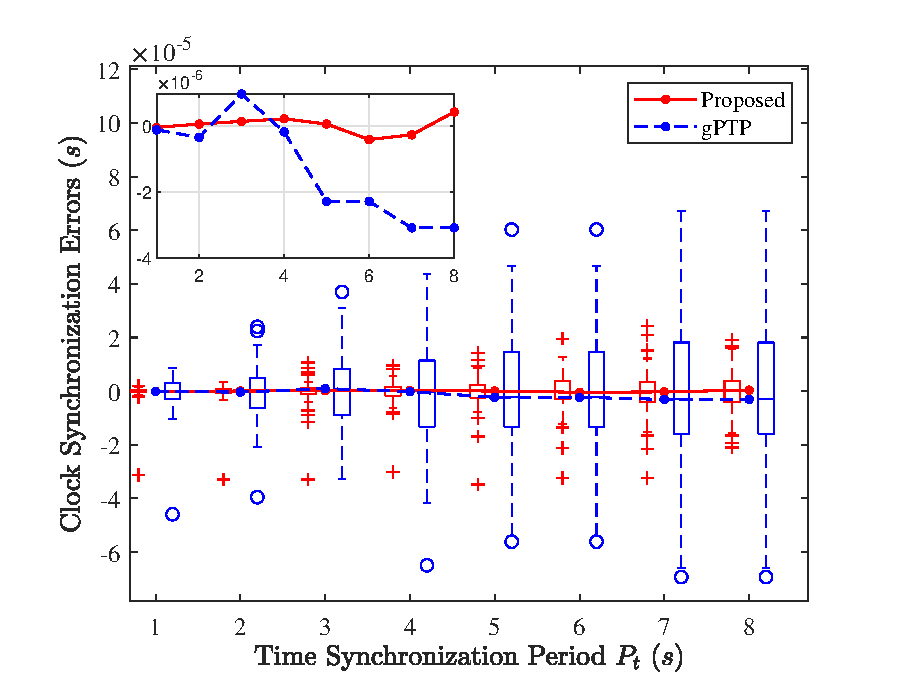
\includegraphics[scale=0.6]{fig7.eps}}
	\caption{Synchronization errors comparison of two methods with different $P_t$.}
	\label{fig7}
\end{figure}

\subsection{Synchronization Speed}
Fig. 8 shows the synchronization speed of the two mechanisms with different $P_t$. We define the synchronization speed as the time when the relative error between the current synchronization accuracy and the median synchronization accuracy is $20\%$. It can be observed from the figure that the time required for our proposed mechanism is shorter than gPTP, which means that the synchronization speed of our proposed mechanism is faster and synchronization efficiency is higher than gPTP. The synchronization speed of gPTP is slow because it requires multiple cycles of synchronization to eliminate the errors gradually. Moreover, the frequency offset will continue to bring errors, resulting in a long time to achieve the required synchronization accuracy. Our method relies on the SM to provide a reference clock to eliminate errors at the beginning of synchronization quickly. After frequency synchronization, the errors become smaller, so that the synchronization accuracy is always kept in a low range.

\begin{figure}[t]
	\centerline{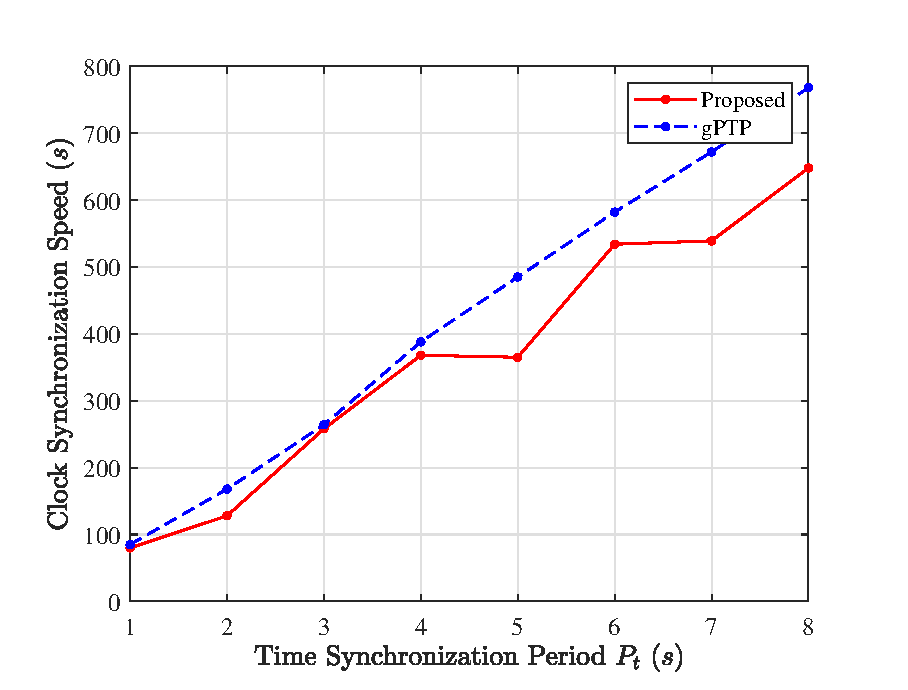
\includegraphics[scale=0.6]{fig8.eps}}
	\caption{Synchronization speed comparison of two methods with different $P_t$.}
	\label{fig8}
\end{figure}

\subsection{Performance Analysis}
The synchronization mechanism proposed in this work adopts a hierarchical structure. Since all SMs are synchronized with GM, the calculation of the underlying network can eliminate random errors. Moreover, due to the combination of distributed synchronization, which avoids the situation that tree-based synchronization errors will accumulate as the network scale increases, the synchronization process can be increased compared to gPTP with the same synchronization period. It can achieve the required synchronization accuracy faster, resulting in higher synchronization efficiency, which can also be seen from Fig. 8. 

%\subsection{Reliability}
%Fig. 9 shows the tendency of the synchronization accuracy of the two synchronization mechanisms under abnormal GM conditions. At the beginning of the figure, both mechanisms work normally. However, assuming that the GM is abnormal in the middle, we find that the synchronization accuracy of PTP will be severely affected later, but the synchronization mechanism proposed in this paper can still guarantee high synchronization accuracy. This is because we designed an exception judgment mechanism during synchronization to ensure the reliability of synchronization.

\section{Conclusions}
This paper has studied the clock synchronization for TSN. A hierarchical clock synchronization mechanism was proposed. Considering the synchronization time slot difference and the time-frequency coupling relationship, the offset of time and frequency are cooperatively regulated. Through the performance analysis and verification, the effectiveness and performance improvement of the proposed hierarchical synchronization mechanism was demonstrated. In the future, we will do further research on synchronization reliability.

\section*{Acknowledgment}
This work was supported  by National Key Research and Development Program of China (2018YFB1702100).

%\begin{thebibliography}{00}
%\bibitem{b1} G. Eason, B. Noble, and I. N. Sneddon, ``On certain integrals of Lipschitz-Hankel type involving products of Bessel functions,'' Phil. Trans. Roy. Soc. London, vol. A247, pp. 529--551, April 1955.
%\bibitem{b2} J. Clerk Maxwell, A Treatise on Electricity and Magnetism, 3rd ed., vol. 2. Oxford: Clarendon, 1892, pp.68--73.
%\bibitem{b3} I. S. Jacobs and C. P. Bean, ``Fine particles, thin films and exchange anisotropy,'' in Magnetism, vol. III, G. T. Rado and H. Suhl, Eds. New York: Academic, 1963, pp. 271--350.
%\bibitem{b4} K. Elissa, ``Title of paper if known,'' unpublished.
%\bibitem{b5} R. Nicole, ``Title of paper with only first word capitalized,'' J. Name Stand. Abbrev., in press.
%\bibitem{b6} Y. Yorozu, M. Hirano, K. Oka, and Y. Tagawa, ``Electron spectroscopy studies on magneto-optical media and plastic substrate interface,'' IEEE Transl. J. Magn. Japan, vol. 2, pp. 740--741, August 1987 [Digests 9th Annual Conf. Magnetics Japan, p. 301, 1982].
%\bibitem{b7} M. Young, The Technical Writer's Handbook. Mill Valley, CA: University Science, 1989.
%\end{thebibliography}

\bibliographystyle{IEEEtran}
\bibliography{REF}

\end{document}